		
%% bare_conf.tex
%% V1.4b
%% 2015/08/26
%% by Michael Shell
%% See:
%% http://www.michaelshell.org/
%% for current contact information.
%%
%% This is a skeleton file demonstrating the use of IEEEtran.cls
%% (requires IEEEtran.cls version 1.8b or later) with an IEEE
%% conference paper.
%%
%% Support sites:
%% http://www.michaelshell.org/tex/ieeetran/
%% http://www.ctan.org/pkg/ieeetran
%% and
%% http://www.ieee.org/

%%*************************************************************************
%% Legal Notice:
%% This code is offered as-is without any warranty either expressed or
%% implied; without even the implied warranty of MERCHANTABILITY or
%% FITNESS FOR A PARTICULAR PURPOSE! 
%% User assumes all risk.
%% In no event shall the IEEE or any contributor to this code be liable for
%% any damages or losses, including, but not limited to, incidental,
%% consequential, or any other damages, resulting from the use or misuse
%% of any information contained here.
%%
%% All comments are the opinions of their respective authors and are not
%% necessarily endorsed by the IEEE.
%%
%% This work is distributed under the LaTeX Project Public License (LPPL)
%% ( http://www.latex-project.org/ ) version 1.3, and may be freely used,
%% distributed and modified. A copy of the LPPL, version 1.3, is included
%% in the base LaTeX documentation of all distributions of LaTeX released
%% 2003/12/01 or later.
%% Retain all contribution notices and credits.
%% ** Modified files should be clearly indicated as such, including **
%% ** renaming them and changing author support contact information. **
%%*************************************************************************


% *** Authors should verify (and, if needed, correct) their LaTeX system ***
% *** with the testflow diagnostic prior to trusting their LaTeX platform ***
% *** with production work. The IEEE's font choices and paper sizes can ***
% *** trigger bugs that do not appear when using other class files. *** ***
% The testflow support page is at:
% http://www.michaelshell.org/tex/testflow/



\documentclass[conference]{IEEEtran}
% Some Computer Society conferences also require the compsoc mode option,
% but others use the standard conference format.
%
% If IEEEtran.cls has not been installed into the LaTeX system files,
% manually specify the path to it like:
% \documentclass[conference]{../sty/IEEEtran}





% Some very useful LaTeX packages include:
% (uncomment the ones you want to load)


% *** MISC UTILITY PACKAGES ***
%
%\usepackage{ifpdf}
% Heiko Oberdiek's ifpdf.sty is very useful if you need conditional
% compilation based on whether the output is pdf or dvi.
% usage:
% \ifpdf
% % pdf code
% \else
% % dvi code
% \fi
% The latest version of ifpdf.sty can be obtained from:
% http://www.ctan.org/pkg/ifpdf
% Also, note that IEEEtran.cls V1.7 and later provides a builtin
% \ifCLASSINFOpdf conditional that works the same way.
% When switching from latex to pdflatex and vice-versa, the compiler may
% have to be run twice to clear warning/error messages.






% *** CITATION PACKAGES ***
%
%\usepackage{cite}
% cite.sty was written by Donald Arseneau
% V1.6 and later of IEEEtran pre-defines the format of the cite.sty package
% \cite{} output to follow that of the IEEE. Loading the cite package will
% result in citation numbers being automatically sorted and properly
% "compressed/ranged". e.g., [1], [9], [2], [7], [5], [6] without using
% cite.sty will become [1], [2], [5]--[7], [9] using cite.sty. cite.sty's
% \cite will automatically add leading space, if needed. Use cite.sty's
% noadjust option (cite.sty V3.8 and later) if you want to turn this off
% such as if a citation ever needs to be enclosed in parenthesis.
% cite.sty is already installed on most LaTeX systems. Be sure and use
% version 5.0 (2009-03-20) and later if using hyperref.sty.
% The latest version can be obtained at:
% http://www.ctan.org/pkg/cite
% The documentation is contained in the cite.sty file itself.






% *** GRAPHICS RELATED PACKAGES ***
%
\ifCLASSINFOpdf
 % \usepackage[pdftex]{graphicx}
 % declare the path(s) where your graphic files are
 % \graphicspath{{../pdf/}{../jpeg/}}
 % and their extensions so you won't have to specify these with
 % every instance of \includegraphics
 % \DeclareGraphicsExtensions{.pdf,.jpeg,.png}
\else
 % or other class option (dvipsone, dvipdf, if not using dvips). graphicx
 % will default to the driver specified in the system graphics.cfg if no
 % driver is specified.
 % \usepackage[dvips]{graphicx}
 % declare the path(s) where your graphic files are
 % \graphicspath{{../eps/}}
 % and their extensions so you won't have to specify these with
 % every instance of \includegraphics
 % \DeclareGraphicsExtensions{.eps}
\fi
% graphicx was written by David Carlisle and Sebastian Rahtz. It is
% required if you want graphics, photos, etc. graphicx.sty is already
% installed on most LaTeX systems. The latest version and documentation
% can be obtained at: 
% http://www.ctan.org/pkg/graphicx
% Another good source of documentation is "Using Imported Graphics in
% LaTeX2e" by Keith Reckdahl which can be found at:
% http://www.ctan.org/pkg/epslatex
%
% latex, and pdflatex in dvi mode, support graphics in encapsulated
% postscript (.eps) format. pdflatex in pdf mode supports graphics
% in .pdf, .jpeg, .png and .mps (metapost) formats. Users should ensure
% that all non-photo figures use a vector format (.eps, .pdf, .mps) and
% not a bitmapped formats (.jpeg, .png). The IEEE frowns on bitmapped formats
% which can result in "jaggedy"/blurry rendering of lines and letters as
% well as large increases in file sizes.
%
% You can find documentation about the pdfTeX application at:
% http://www.tug.org/applications/pdftex





% *** MATH PACKAGES ***
%
%\usepackage{amsmath}
% A popular package from the American Mathematical Society that provides
% many useful and powerful commands for dealing with mathematics.
%
% Note that the amsmath package sets \interdisplaylinepenalty to 10000
% thus preventing page breaks from occurring within multiline equations. Use:
%\interdisplaylinepenalty=2500
% after loading amsmath to restore such page breaks as IEEEtran.cls normally
% does. amsmath.sty is already installed on most LaTeX systems. The latest
% version and documentation can be obtained at:
% http://www.ctan.org/pkg/amsmath





% *** SPECIALIZED LIST PACKAGES ***
%
%\usepackage{algorithmic}
% algorithmic.sty was written by Peter Williams and Rogerio Brito.
% This package provides an algorithmic environment fo describing algorithms.
% You can use the algorithmic environment in-text or within a figure
% environment to provide for a floating algorithm. Do NOT use the algorithm
% floating environment provided by algorithm.sty (by the same authors) or
% algorithm2e.sty (by Christophe Fiorio) as the IEEE does not use dedicated
% algorithm float types and packages that provide these will not provide
% correct IEEE style captions. The latest version and documentation of
% algorithmic.sty can be obtained at:
% http://www.ctan.org/pkg/algorithms
% Also of interest may be the (relatively newer and more customizable)
% algorithmicx.sty package by Szasz Janos:
% http://www.ctan.org/pkg/algorithmicx




% *** ALIGNMENT PACKAGES ***
%
%\usepackage{array}
% Frank Mittelbach's and David Carlisle's array.sty patches and improves
% the standard LaTeX2e array and tabular environments to provide better
% appearance and additional user controls. As the default LaTeX2e table
% generation code is lacking to the point of almost being broken with
% respect to the quality of the end results, all users are strongly
% advised to use an enhanced (at the very least that provided by array.sty)
% set of table tools. array.sty is already installed on most systems. The
% latest version and documentation can be obtained at:
% http://www.ctan.org/pkg/array


% IEEEtran contains the IEEEeqnarray family of commands that can be used to
% generate multiline equations as well as matrices, tables, etc., of high
% quality.




% *** SUBFIGURE PACKAGES ***
%\ifCLASSOPTIONcompsoc
% \usepackage[caption=false,font=normalsize,labelfont=sf,textfont=sf]{subfig}
%\else
% \usepackage[caption=false,font=footnotesize]{subfig}
%\fi
% subfig.sty, written by Steven Douglas Cochran, is the modern replacement
% for subfigure.sty, the latter of which is no longer maintained and is
% incompatible with some LaTeX packages including fixltx2e. However,
% subfig.sty requires and automatically loads Axel Sommerfeldt's caption.sty
% which will override IEEEtran.cls' handling of captions and this will result
% in non-IEEE style figure/table captions. To prevent this problem, be sure
% and invoke subfig.sty's "caption=false" package option (available since
% subfig.sty version 1.3, 2005/06/28) as this is will preserve IEEEtran.cls
% handling of captions.
% Note that the Computer Society format requires a larger sans serif font
% than the serif footnote size font used in traditional IEEE formatting
% and thus the need to invoke different subfig.sty package options depending
% on whether compsoc mode has been enabled.
%
% The latest version and documentation of subfig.sty can be obtained at:
% http://www.ctan.org/pkg/subfig




% *** FLOAT PACKAGES ***
%
%\usepackage{fixltx2e}
% fixltx2e, the successor to the earlier fix2col.sty, was written by
% Frank Mittelbach and David Carlisle. This package corrects a few problems
% in the LaTeX2e kernel, the most notable of which is that in current
% LaTeX2e releases, the ordering of single and double column floats is not
% guaranteed to be preserved. Thus, an unpatched LaTeX2e can allow a
% single column figure to be placed prior to an earlier double column
% figure.
% Be aware that LaTeX2e kernels dated 2015 and later have fixltx2e.sty's
% corrections already built into the system in which case a warning will
% be issued if an attempt is made to load fixltx2e.sty as it is no longer
% needed.
% The latest version and documentation can be found at:
% http://www.ctan.org/pkg/fixltx2e


%\usepackage{stfloats}
% stfloats.sty was written by Sigitas Tolusis. This package gives LaTeX2e
% the ability to do double column floats at the bottom of the page as well
% as the top. (e.g., "\begin{figure*}[!b]" is not normally possible in
% LaTeX2e). It also provides a command:
%\fnbelowfloat
% to enable the placement of footnotes below bottom floats (the standard
% LaTeX2e kernel puts them above bottom floats). This is an invasive package
% which rewrites many portions of the LaTeX2e float routines. It may not work
% with other packages that modify the LaTeX2e float routines. The latest
% version and documentation can be obtained at:
% http://www.ctan.org/pkg/stfloats
% Do not use the stfloats baselinefloat ability as the IEEE does not allow
% \baselineskip to stretch. Authors submitting work to the IEEE should note
% that the IEEE rarely uses double column equations and that authors should try
% to avoid such use. Do not be tempted to use the cuted.sty or midfloat.sty
% packages (also by Sigitas Tolusis) as the IEEE does not format its papers in
% such ways.
% Do not attempt to use stfloats with fixltx2e as they are incompatible.
% Instead, use Morten Hogholm'a dblfloatfix which combines the features
% of both fixltx2e and stfloats:
%
% \usepackage{dblfloatfix}
% The latest version can be found at:
% http://www.ctan.org/pkg/dblfloatfix




% *** PDF, URL AND HYPERLINK PACKAGES ***
%
%\usepackage{url}
% url.sty was written by Donald Arseneau. It provides better support for
% handling and breaking URLs. url.sty is already installed on most LaTeX
% systems. The latest version and documentation can be obtained at:
% http://www.ctan.org/pkg/url
% Basically, \url{my_url_here}.




% *** Do not adjust lengths that control margins, column widths, etc. ***
% *** Do not use packages that alter fonts (such as pslatex). ***
% There should be no need to do such things with IEEEtran.cls V1.6 and later.
% (Unless specifically asked to do so by the journal or conference you plan
% to submit to, of course. )


% correct bad hyphenation here
\hyphenation{op-tical net-works semi-conduc-tor}
\usepackage{graphicx}
\usepackage{verbatim}
\usepackage{array}
\usepackage{filecontents}
\usepackage{caption}
\usepackage[noadjust]{cite}
\captionsetup[table]{position=bottom} %% or below

\begin{document}
%
% paper title
% Titles are generally capitalized except for words such as a, an, and, as,
% at, but, by, for, in, nor, of, on, or, the, to and up, which are usually
% not capitalized unless they are the first or last word of the title.
% Linebreaks \\ can be used within to get better formatting as desired.
% Do not put math or special symbols in the title.
\title{Precise Weed and Maize classification through Convolutional Neuronal Networks }


% author names and affiliations
% use a multiple column layout for up to three different
% affiliations
\author{\IEEEauthorblockN{Andrea Concepci\'on C\'ordova Cruzatty \IEEEauthorrefmark{1},
Mauricio Daniel Barreno Barreno \IEEEauthorrefmark{2} and Jos\'e Misael J\'acome Barrionuevo\IEEEauthorrefmark{3}}
\IEEEauthorblockA{Department of Energy and Mechanics,
University of the Army ESPE\\
Latacunga - Quijano y Ordo\~nez and Hermanas Pa\'ez \\
Email: \IEEEauthorrefmark{1}accordova@espe.edu.ec,
\IEEEauthorrefmark{2}mdbarreno@espe.edu.ec,
\IEEEauthorrefmark{3}jmjacome1@espe.edu.ec}}
% conference papers do not typically use \thanks and this command
% is locked out in conference mode. If really needed, such as for
% the acknowledgment of grants, issue a \IEEEoverridecommandlockouts
% after \documentclass

% for over three affiliations, or if they all won't fit within the width
% of the page, use this alternative format:
% 
%\author{\IEEEauthorblockN{Michael Shell\IEEEauthorrefmark{1},
%Homer Simpson\IEEEauthorrefmark{2},
%James Kirk\IEEEauthorrefmark{3}, 
%Montgomery Scott\IEEEauthorrefmark{3} and
%Eldon Tyrell\IEEEauthorrefmark{4}}
%\IEEEauthorblockA{\IEEEauthorrefmark{1}School of Electrical and Computer Engineering\\
%Georgia Institute of Technology,
%Atlanta, Georgia 30332--0250\\ Email: see http://www.michaelshell.org/contact.html}
%\IEEEauthorblockA{\IEEEauthorrefmark{2}Twentieth Century Fox, Springfield, USA\\
%Email: homer@thesimpsons.com}
%\IEEEauthorblockA{\IEEEauthorrefmark{3}Starfleet Academy, San Francisco, California 96678-2391\\
%Telephone: (800) 555--1212, Fax: (888) 555--1212}
%\IEEEauthorblockA{\IEEEauthorrefmark{4}Tyrell Inc., 123 Replicant Street, Los Angeles, California 90210--4321}}




% use for special paper notices
%\IEEEspecialpapernotice{(Invited Paper)}




% make the title area
\maketitle

% As a general rule, do not put math, special symbols or citations
% in the abstract
\begin{abstract}

Deep Learning has played a very important role in modern times, being very used in Artificial Vision and especially in Pattern Recognition, which opens many doors in the fields of application among which is precision agriculture. In this paper the study of a convolutional neural network is presented, with two classes applied to the classification of plants of maize and weeds in real time, focused to fields of maize in its initial stage. The algorithm has two stages, segmentation of images and classification. Segmentation is intended to separate the target plant from the original image. While the classification is possible through a convolutional neural network, previously trained with a dataset generated through the segmentation stage. The performance of the network is illustrated by analysis and comparisons with different network architectures, then with the network that presented better results in training, (revisar esta linea) we experimented by modifying its number of filters, to analyze their behavior. Finally, the resulting network was tested on different processors to compare classification times.\\

\begin{comment}
-Deep Learning ha tenido un papel muy importante en los tiempos modernos, siendo muy utilizado en vision artificial y especialmente en reconocimiento de patrones, lo cual abre muchas puertas en los campos de aplicacion siendo uno de ellos la agricultura de presicion.En este paper presentamos el estudio una red neuronal convolucional aplicada a la clasificacion de plantas de maiz y de mala hierba en tiempo real, dirigida a campos de maiz en su etapa inicial.El algoritmo cuenta con dos etapas, segmentacion de imagenes y la clasificacion. En la segmentacion se busca separar de la imagen las plantas de forma individual. Mientras que la clasificacion se da a traves de la red neuronal convolucional, previamente entrenada con un dataset generado mediante la etapa de segmentacion. El rendimiento de la red se ilustra mediante analisis y comparaciones con diferentes arquitecturas de red, luego con la red que presento mejores resultados, se experimeto modificando su numero de filtros, para analizar su comportamiento. Finalmente con la red resultante se implemet\'o en diferentes procesadores para comparar tiempos de clasificacion.
\end {comment}
\end{abstract}

% no keywords




% For peer review papers, you can put extra information on the cover
% page as needed:
% \ifCLASSOPTIONpeerreview
% \begin{center} \bfseries EDICS Category: 3-BBND \end{center}
% \fi
%
% For peerreview papers, this IEEEtran command inserts a page break and
% creates the second title. It will be ignored for other modes.
\IEEEpeerreviewmaketitle

\section{Introduction}
During the last centuries, significant progress has taken place in science and technology developments. Significant milestones in diverse areas such as communications, numerical computer control and the miniaturization of components have benefited industrial sectors, providing new means to approach problems in a different manner. 
\\

The availability of leading edge technologies has considerably increased, thus becoming more accessible to people. This effect of globalization has allowed many countries to have access to state-of-the-art technological products, promoting its application in different areas to generate alternative and more efficient solutions to conventional problems. 
\\

Technological advances have caused industry transformations; manufacturing, food processing, and information industries among others, have gone through dramatic changes with industrial revolution. However there are fields that have not been significantly influenced by technological development in Ecuador, as it is the case of agroindustry. Agriculture in Ecuador has undergone some changes since colonial times; while it is true that there are efficient agricultural practices, the lack of technological resources make it impossible for the country to exploit its true potential as an agricultural producer. Also, the excessive use of pesticides have a negative effect on the production, soil, and water quality. 
\\

Nowadays, one of agriculture's challenges is the development of precision agriculture techniques focused on Weed and Crop segmentation. There are studies that show the impact of Weed in corn crops \cite{suarez2005distintos}; its yield is affected by 5000 kg/ha. Currently, growing development of Artificial Vision and Machine Learning algorithms allow researchers to propose solutions for Weed Segmentation in Crops. 
\\

One of the first approximations to the algorithms of detection of Crops was developed in 1996 \cite{brivot1996segmentation}, this algorithm permitted to segment crops from weed, it could be possible by the use of IR Images, the image is processed by a hysteresis umbral and the method of Min Neighbouring to identify the row of crops. In recent years the implementation of Machine Learning has opened new possibilities for differentiate the Weed from the crops, recently \cite{cheng2015feature} there had been developed an algorithm by the use of Harris Corner detector, Feature Detector and using the DBSCAN (Density-based spartial clustering of apllications with noise) , it demonstrates an effectiveness of 98\% in the identification of Weeds in the Rice, Araguez \textit{et. al} \cite{equipo2006proceedings} performed their segmentation through the analysis of the green hystogram and performing the segmentation of the crop and weed by classifiers not specified in the document. 
\\

Hong and Lei \cite{jeon2011robust} developed their approximation by using an optimal method for detection in various types of luminosity, they achived this by the use an ANN for weed and maize classification, with a precision of 92.5\%, also there had been developed an algorithm \cite{hlaing2014weed}, that through binarization methods of OTSU and Watershed for the segmentation of the images. While its classification was given through an areas analysis to perform a thresholding, although the method is computationally effective when the Weed distribution does not resemble the size to the crop plant, its error increases when there is more density of crop than of weed. Romeo \textit{et. al} \cite{romeo2012crop} propose to use a fuzzy clustering approach to correctly segment the crop green.
\\

The segmentation of weed and crops is not closed to color images, using a multispectral camera \cite{potena2016fast} permitted to obtain RGB and NIR images, for the segmentation and classification, then the images used a light CNN for the first process and a Deep CNN for classification in Crops, its accuracy is up to 98\% in the identification of weeds. One of the most dificults things for the identification of crops is the generation of Datasets due to presence of Weed in the images of training, but there could be correctly generated by a Convolutional Neural Network \cite{di2016automatic} achieving a acceptable accuracy for the generation of Datasets. 
\\

\section{Matherials and Methods}
\begin{comment}
El desarrollo del modelo para la identificacion de mala hierba y maiz usando Redes Neuronales Convoluciones se describe abajo: 
\end{comment}

The model development for weed and maize identification algorithm using convolutional neural networks is described below.
\\
\subsection{Hardware}
\begin{comment}
Para la etapa de entranamiento y captura de imagenes, los siguientes elementos fueron utilizados: Una Raspberry Pi 3 con su modulo de camara V2.1 para la adquisicion de imagenes, fue configurado para obtener video en resolucion de 1280x720 pixeles con el fin de obtener mayor detalle en la segmentacion de imagenes. Debido a la popularidad de la computacion por GPU(IDEA COMPLETADA) por sus ventajas en el desarrollo de modelos de Redes Neuronales Convolucionales, fue necesario consider hardware compatible con computacion paralela como las tarjetas graficas fabricadas por NVIDIA, estas tienen la ventaja de poseer mejores tiempos de procesamiento comparados con la CPU, con lo cual se logra optimizar los tiempos de clasificacion y entrenamiento de Modelos de Deep Learning, entonces, utilizamos un computador con una tarjeta Grafica NVIDIA GTX950M. Tambien fue necesario considerar el uso de un CPU Core i7 2.7Ghz, 8 Nucles and el CPU de la propia Raspberry Pi 3, un ARM 3, a ARM Cortex-A53, 1.2GHz, 4 nucles para probar el rendimiento de red en un sistema portable para su aplicacion en un sistema movil independiente . El hardware escogido sera probado para clasificar las imagenes y medir los tiempos de clasificacion para su posterior analisis. El hardware elegido será probado para clasificar imágenes, en cada clasificación se medirán los tiempos de procesamiento, para realizar un análisis si el hardware puede procesar en tiempo real 
\end{comment}

For the training and image-capturing stages, the following elements were used: a Raspberry Pi 3 with a V2.1 Pi camera for image acquisition. The system was configured to obtain a video at a resolution of 1280x720 pixels in order to get more detail in the segmented images. Due to the popularity of GPU computing for its advantages in the development of models of Convolutional Neural Networks (COMPLETAR IDEA), it was necessary to consider hardware compatible with parallel computing such as the Graphic Cards manufactured by NVIDIA. These cards have the advantage of a superior processing speed compared to a CPU in order to optimize image-processing time and deep learning Model's training process, thus the selected device was a computer with a Nvidia graphics card GTX950M. Also, it was necessary to consider the use of a Core i7 2.7 Ghz CPU of 8 cores and the CPU of the Raspberry Pi 3, an ARM Cortex-A53, 1.2GHz, 4 cores (CLARIFICAR IDEA) for test its performance in this embedded system for a future aplication in a independent mobile system. The hardware chosen will be tested to classify images, in each classification  a measure the times of processing will be performed, for make an analysis if the hardware can process in real time. 
\\

\subsection{Software}
\begin{comment}
Para la aplicacion en este documento, se requiere el uso de Poderosas librerias de desarrollo para el procesamiento de imagenes y Deep Learning, fueron requeridas debido a que se necesita de Vision Artificial para realizar la segmentacion de plantas del suelo y generar imagenes independientes de cada una y la otra libreria sirve para la clasificacion de las imagenes obtenidas y su analisis de precision en diferentes arquitecturas de red con el fin de elegir la mas adecuada para nuestro proposito. Consideramos el uso de software libre para extender su uso en futuros prototipos, debido a esta consideracion hemos escogido la libreria de OpenCV debido a su eficiencia computacional y su enfoque a aplicaciones en tiempo real, para este caso fue utilizada(en referencia a OpenCV) para la adquisicion y segmentacion de las imagenes de muestra. Tambien hemos considerado Caffe debido a que esta desstinado a el entrenamiento y desarrollo de Redes Neuronales Convolucionales de Proposito General y otros modelos de Deep Learning con soporte completo de la Libreria de Computacion GPU CUDA y una generosa base de datos de recursos para aprendizaje de aplicaciones como Simple Regresion, Robotica, large-scale visual classification, etc. 
\end{comment}

The use of powerful libraries of Image Processing and Deep Learning Development was required due to.... . The use of open software was required in order to provide the system with a certain level of flexibility to extend its use for future prototypes. Thus, OpenCV library was chosen due to its computational efficiency and focus on real-time applications \cite{opencv_library}; it was used specificaly for sample images acquisition and segmentation. Also, Caffe was considered because it is intended to aid in the training and developing of general-purpose convolutional neural networks and other Deep Lerning models \cite{jia2014caffe} with full support of CUDA GPU computation library and a generous database of resources for learning of applications such as simple regression, speech, robotics, large-scale visual classification, etc.	
\\
\begin{comment}
Tambien el la etapa de desarrollo fue importante el suo del Sistema Operativo Linux, sus caracteristicas son: Sistema Operativo Ligero y Libre tambien completamente compatible con el software mencionado anteriormente. En la computadora principal fue usado la Distribucion Ubuntu Linux 16.04 por su soporte oficial a CUDA, Caffe y OpenCV, tambien en la Raspberry Pi fue usado el Sistema Operativo Pixel para adquirir imagenes y probar el rendimiento de clasificacion la Red Neuronal Convolucional
\end{comment}

Also in the development stage was important the use of Linux OS , its features are: lightweight and free OS also fully compatible with the software mentioned above. For the main computer was used Ubuntu Linux 16.04 for its official support to CUDA, Caffe and OpenCV, also in the Raspberry Pi the Pixel OS was used for acquire images and test the classification performace of the CNN.
\\

\subsection{Dataset Description}
\begin{comment}
Debido a la falta de datasets de plantas de Maize y Mala Hierba, Fue necesario buscar los cultivos de maíz en su etapa de desarrollo inicial porque las acciones tomadas en esta etapa por el agricultor tendrán un impacto en el rendimiento futuro del cultivo, para ese proposito nos hemos traslatado a Pillaro, esta ciudad es localizada en la Provincia de Tungurahua, en el Centro de la Sierra Ecuatoriana. Pillaro es un productor reconocido de cultivos andinos como: Maiz, Papas y frutas, por lo que podemos encontrar aqui muchos cultivos de maiz que sean utiles para nuestro proposito
\begin{comment}

Due to the lack of weed and maize plant datasets, it was necessary to search maize crops in its initial development stage because the taken actions in this stage by the farmer will impact in the future yield of the crop (IDEA COMPLETADA). Fieldwork at a nearby town called P\'illaro was arranged with the purpose of obtaining image samples. P\'illaro it is a city located in the Tungurahua Province, in the center of the Ecuadorian Highlands region, it is a recognized andean-crop producer of species such as: maize, potatoes and a wide variety of fruits. Due to its year-long production season, many maize crops at its initial development stage were found in this area. \\

\begin{comment}
Las muestras fueron obtenidas de imagenes capturas en esos campos de maiz, consideramos escoger cultivos de maiz donde podamos visualmente discrimiar las plantas del cultivo de la mala yerba para para facilitar la segmentacion de las imágenes y para proporcionar a red de muestras confiables que permiten al modelo aprender correctamente todas las características de la planta real. Las etapas del Maiz (V3-V7) fueron usadas para tomar muestras. Para obtener las muestra, centramos la camara sobre la platna objetivo, asegurandonos que la captura muestre todas las caracteristicas de la planta de maiz, esto fue posible al monitorear el proceso por una pantalla externa. Unas muestras de las imagenes capturadas son mostradas a continuacion: 
\begin{comment}


Samples were obtained from images captured in different maize fields. Crops were weed and maize plants could be visually discriminated were chosen in order to easy segment the images and for provide to Net of reliable samples which permit to the model to correctly learn all features of the real plant (IDEA SUSTENDAD). Maize Plants at a V3 to V7 develompent stage (3-7 leafs) \cite{fassio1998maiz} were used to take samples. To record the samples, a camera was centered over the target plant, insuring that the capture shows all features of the maize plant. This was achieved by monitoring the obtained samples through an external display. Examples of the images captured are shown below. 


	\begin{figure}[h]
	\centering
	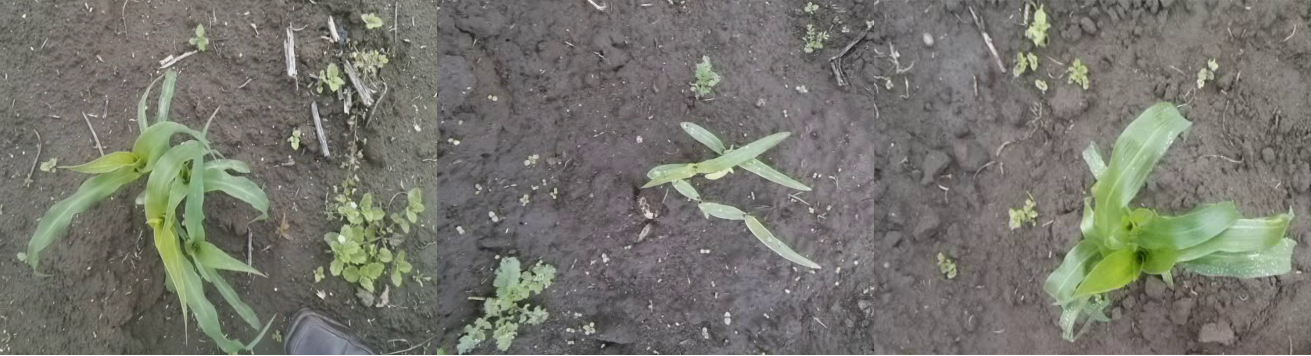
\includegraphics[width=3.2in]{entradamaiz}
	\caption{Crops chosen to obtain samples, notice that it is easy to discrimante weed from maize}
	\label{fig_sim}
	\end{figure}
\begin{comment}
Tambien fue necesario obtener imagenes de las malas hierbas mas comunes en los campos de maiz de Pillaro, para permitir a la Red discrimiar entre las dos clases definidas en el Dataset.
\end{comment}

Also, it was necessary to obtain images of the most common weed plants of the maize crops in Pillaro, to allow the network to discriminate between the two defined classes of the dataset. \\
\begin{comment}
Entonces, a traves de un proceso de procesamiento digital de imagenes, como primera fase, la imagen fue normalizada en su canal verde, esto mejora la deteccion del color verde porque elimina las luces y las sombras de la imagen, despues extrajimos el color verde de la imagen con la ecuacion descrita opr Wang, Men, Luo and Mei, para obtener una imagen final en escala de grises, despues se aplico una Umbralizacion de OTSU para obtener una mascara binaria 
\end{comment}
	
Then, through a first-stage digital image processing procedure, the images were normalized in its green channel. This was done in order to improve green color detection based on the elimination of light and shadow in the images. Later, the green color was extracted from the images to obtain a grayscale equivalent; this was done through the following equation described by Wang, Meng, Luo and Mei \cite{wang2013path}. Following, an OTSU Thresholding was applied to the grayscale images in order to obtain a binary mask. 
\begin{equation}
	S = 2*G - R - B
\end{equation} 
\begin{comment}
Despues de la imagen fue segmentada, para diferenciarla del suelo y otros elementos que no sean plantas, las imagenes originales fueron enmascaradas con la mascara binaria para proveer al Dataset caracteristicas de Color del Maiz y de la Mala Hierba. Una vez ue las imagenes segmentedas fueron obtenidas, removimos aquellas que tenian una resolucion menor a 64x64 pixeles debido a que son mas pequenhas que el tamanho de entrada de la red, ademas no es conveniente procesarlas debido a que su area total es mucho mas pequenha que la de las muestras de maiz, las cuales son el proposito de este documento, despues las imagenes se almacenan en un formato Png. El proceso se ilustra de mejor manera en la siguiente figura.
\end{comment}

Afterwards, the images were segmented in order to differentiate them from the soil and other non-plant elements. Original images were masked with the binary mask to provide the dataset with color features of maize and weed plants. Once the segmented images were obtained, images that had a resolution lower than 64x64 pixels were removed because its size was smaller than the size of the network input layer. Besides, the processing of these small images was not convenient since its total area was much smaller than the maize sample images. Following, the images were saved in a png format. The entire process described before is illustrated in the next figure. \\

	\begin{figure}[h]
	\centering
	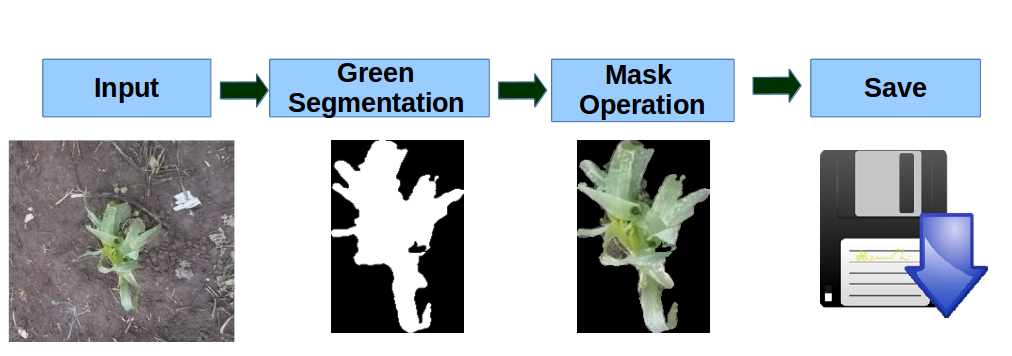
\includegraphics[width=3.2in]{procesamiento}
	\caption{Preprocessing to obtain samples for the dataset}
	\label{fig_sim}
	\end{figure}

\begin{comment}	
Debemos acotar que hemos etiquetado manualmente las imagenes en dos clases, maiz y mala hierba, teniendo en cuenta que las imagenes no se repitan(\textbf{corregir}). En la presente imagen presentamos los resultados finales de las imagenes procesadas que conforman el dataset. 
\end{comment}

It should be noted that samples were manually labeled into two classes; maize and weed, making sure that the images are not repeated. In the following image, final results of the processed images that conform the dataset are shown.\\
	
	\begin{figure}[h]
	\centering
	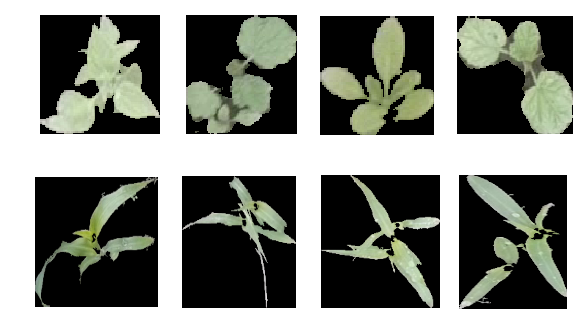
\includegraphics[width=2.5in]{im1}
	\caption{ Segmented and Masked images of dataset Above: Weed, Below: Maize}
	\label{fig_sim}
	\end{figure}

\begin{comment}	
Una vez completada el procesamiento de imagenes, donde fueron obtenidas 2835 imagenes de maiz y 880 images de Mala Hierba, Lee et. Al dicen que una vez que la CNN ha alcanzado una precision aceptable, el dataset se puede extender por transformaciones geometricas, en adicion sladojevic mencionan que esto permite a reducir el sobreajuste y para mejorar la precision en el entrenamiento, razon por la cual hizimos 11 rotaciones cada 30 grados, obteniendo de esta forma el incremento(corregir) del dataset en 12 veces y tener mejores probabilidades de reconocer als plantas en cualquier orientaciones. 
\end{comment}
	
Once image processing was completed, a set of 2835 maize images and 880 weed images was obtained. Lee \textit{et. al} \cite{lee2015deep} said that once CNN has reached an acceptable accuracy, the dataset can be extended by means of geometric transformations. In addition, the geometric transformations \cite{sladojevic2016deep} (Si es verdad) allow overfitting reduction and improves(revisar correspondencia persona) the precision in the training process. For this reason, image rotations each 30 degrees were made, obtaining an increment of the dataset by 12 times, thus increasing the chances of recognizing plants that are in any orientation effectively. \\

\begin{comment}	
Para la fase de validacion, hemos escogido aletariamente la quinta parte del total de imagenes de cada clase, asi que tenemos la siguiente tabla con la distribucion del dataset.
\end{comment}	

For the Validation Phase, a fifth part of the total image set of each class was chosen, resulting in the following chart with the distribution of the dataset.

\begin{table}[h!]
\centering
\begin{tabular}{| c c c c c |} 
 \hline
 \textbf{Phase} & \textbf{Train} & \textbf{Validation} &\textbf{Test} & \textbf{Total} \\ [1ex] 
 \hline
 Maize & 25695 & 8325 & 200 & 34220 \\ 
 Weed & 8560 & 2000 & 200 & 10760\\ 
 \hline
\end{tabular}
\caption{Distribution of the Dataset of each class}
\label{table:1}
\end{table}
	
	
\subsection{Convolutional Neuronal Network}

\begin{comment}	
Despues que el ultimo paso ha sido terminado, fue necesario clasificar las imagenes del Maiz y Mala Hierba, un metodo muy preciso de Clasificacion de Imagenes son las Redes Neuronales Convolucionales(CNN), estos modelos son complejos pero eficientes con un alto grado de discriminacion y han demostrado que tienen unos buenos resultados en la Clasificacion de Imagenes, Deteccion de Objetos y Fine*Grained Classification. Tambien son aplicados en la Agricultura de Precision para la correcta identificacion de plantas
\end{comment}	

	After the dataset was completed, it was neccesary to classify maize and weed images. Convolutional Neural Networks (CNN) can be used as a highly-accurate method for image classification, these models are complex but efficient with a high rate of discrimination and have proven to provide good results in image classification, object detection, and fine-grained classification \cite{sharif2014cnn}. CNN are widely used in precision agriculture \cite{potena2016fast} for the correct identification of plants.\\
	
\begin{comment}	
Una de las caracteristicas de las CNN is que estas pueden tener multiples arquitecturas, cada arquitectura puede alcanzar diferentes resultados dependiendo de la aplicacion, para el presente documento hemos considerado cuatro arquitecturas de CNN: Dos modelos fueron escogidos del Caffe Zoo Model(es un recurso libre liberado por los Desarrolladores de Caffe) Lenet y AlexNet, tambien Potena y Nardi han usado adicionalmente dos tios de modelos, sNET y cNET, estos han sido exitosamente probados en la clasificacion de plantas en cultivos, con las redes secogidas, cada una fue entrenada con un mismo Solver de Tipo AdaDelta, con el mismo Dataset y los resultados del entrenamiento son los siguientes:
\end{comment}	

One of the characteristics of the CNN is that these can have multiple architectures, each architecture can reach different results depending on the application. For the present document four CNN architectures have been considered: two models were chose of the Caffe Zoo Model(it's a free resource provided by Caffe Developers), LeNet and AlexNet also Potena and Nardi had used two additional types of Models, sNET and cNET, they were sucessfully proved in identification of plants in crops\cite{potena2016fast}, with the Nets chosen, each one was trained with a same Solver of type AdaDelta and with the same dataset, the results of training are the following. \\
\begin{table}[h!]
\centering
\begin{tabular}{|l c c c c|} 
 \hline
 \textbf{Parameters }& \textbf{LeNet} & \textbf{AlexNet} & \textbf{cNET} & \textbf{sNET} \\ [0.75ex] 
 \hline
 Input size of images & 32x32 & 64x64 & 64x64 & 64x64 \\ 
 Layers numbers & 9 & 11 & 8 & 4\\
 Number of parameters & 652500 & 20166688 & 6421568 & 135872 \\ 
 Iterations & 3000 & 3000 & 3000 & 3000 \\ 
 Accuracy(\%) & 86.48 & 93.86 & 96.4 & 80.4 \\
 Loss(\%) & 32.80 & 15.32 & 13.72 & 15.32 \\ [1ex] 
 \hline 
\end{tabular}
\caption{Comparison of the 4 types of CNN}
\label{table:2}
\end{table}

\begin{comment}	
Dentro de los parametros mostrados en la Tabla, consideramos la red que alcanze la mas alta tasa de precision y mas baja tasa de perdida, claramente la cNET es la escogida, debido a que esta presenta una precision cercana a la clasificacion humana
\end{comment}	

Within parameters shown on table \ref{table:2}, the network that achieved the highest rate of accuracy and lowest rate of loss was considered; clearly the cNET presented a superior performance due to its near-to-human classification precision.\\

\begin{comment}	
Aunque lo resultados dados de la red fueron excelentes, uno de los propositos principales de este documento es una aproximacion de procesamiento en tiempo real, entonces el numero de parametros a ser computados va a ser un problema, entonces consideramos modificar la red para mejorar el tiempo de procesamiento. Para lograr esto, fue necesario reducir el numero de filtros de cNET de 64 a 16, en la tabla siguiente se muestran los resultados del entrenamiento para los dos tipos de red. 
\end{comment}	
	
Although results given by this type of network are excellent, one of the main purposes of this paper is the implementation of this system in real time. The number of parameters to be computed by the selected network were numerous, so network modifications in order to improve processing time had to be made. To achieve this, it was necessary to reduce the number of filters of cNET from 64 to 16.\\

\begin{table}[h!]
\centering
\begin{tabular}{|l c c |} 
 \hline
 \textbf{Parameters} & \textbf{cNET 16 filters} & \textbf{cNET 64 filters} \\ [0.75ex] 
 \hline
 Number of parameters & 1651376 & 6421568 \\ 
 Iterations & 9000 & 9000 \\ 
 Accuracy(\%) & 97.26 & 96.40 \\
 Loss(\%) & 8.39 & 14.48 \\ [1ex] 
 \hline 
\end{tabular}
\caption{Comparison between cNET of 16 and 64 filters}
\label{table:3}
\end{table}

\begin{comment}	
Esta reduccion permitio reducir el numero de parametros de 1651376(es un 25\% de parametros de la red original), y acerca de la precision d ela red, fue affectada un poco pero asi consigue un 97.2\% de precision en el entrenamiento. 
\end{comment}	

This filter reduction permitted to decrease the number of parameters to 1651376 (this represents only 25\% of the original network parameters) without compromising the network precision in a significant way; it still reached a 97.2\% of accuracy.\\

\begin{comment}	
Entonces el modelo completo de red se forma de la siguiente manera: La capa de entrada que recibe una imagen RGB de 64x64 pixeles, seguida por una capa de convolucion de 16 filtros, un kernel de 5 y stride de 1 pixel, esta capa obtiene solo las principales caracteristicas de la imagen, despues una capa de pooling es aplicada, la cual tiene la funcion de encontrar los maximos valores de las capas, con un tamanho de kernel y stride de 2, despues nuevamente se aplica una segunda capa de convolucion que tiene 16 filtros, ancho de kernel de 5 y un stride de 1, seguido nuevamente de una nueva capa de pooling con un tamanho de kernel y de stride de 2, obteniendo asi una imagen de salida de de tamanho 16x16x16 y finalmente se completa la red con tres capas consecutivas fully-connected, la primera con 384 neuronas, la segunda con 192 y la ultima con dos neuronas que representara la capa las dos clases que se busca clasificar, el modelo resultante se muestra en la siguiente imagen
\end{comment}	

So, the complete network model was conformed by the following components: an input layer where an RGB image of 64x64 pixels is received, followed by a convolution layer of 16 filters, a kernel of 5 and a stride of 1 pixel (this layer only obtains the main characteristics of the image), then a pooling layer is applied, which has the function to find the maximum values of the previous layer with a value of kernel size and stride of 2 (QUE? corregido), then again a second layer of convolution that has 16 filters is applied, the size of kernel is 5 and the stride is 1 (QUE corregido), followed by a new layer of pooling with a kernel size and stride of 2, so the resulting image was has size of 16x16x16. Finally the network is completed with three consecutive fully-connected layers; the first with 384 neurons, the next with 192 and the last with 2 neurons. The type of layers fully-connected contain a total of 478 neurons, where the last two neurons that are the output represent the two classes to identify, the result model is shown in the next graph.\\
	
	\begin{figure}[h]
	\centering
	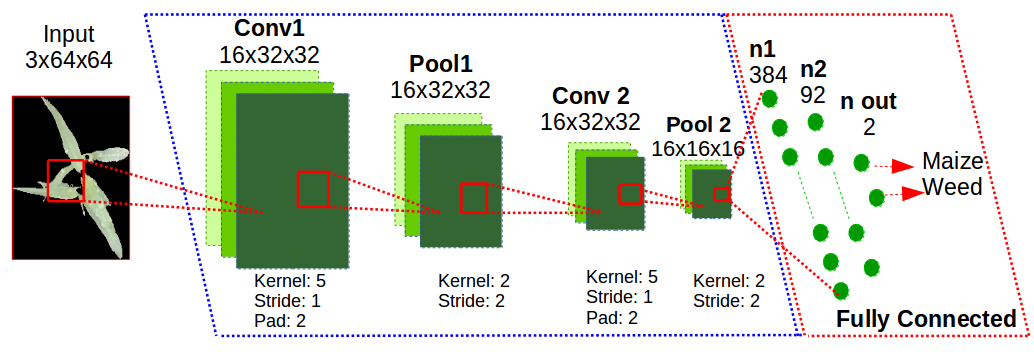
\includegraphics[width=3.5 in]{arquitectura}
	\caption{ The schematic of cNET }
	\label{fig_sim}
	\end{figure}
	
\begin{comment}		
En la grafica de entrenamiento que se muestra a continuacion podemos apreciar el resultado final de precision de la red, la 9000 iteraciones fueron necesarias para reducir el la capa de Loss al minimo y la arquitectura demostro alcanzar rapidamente un valor aceptable de precision, notose que reduciendo el numero de filtros la red gano en precision porque las imagenes del dataset no tienen demasiadas caracteristicas para procesar, por lo que la red fue mejor solucionable con un numero menor parametros de red
\end{comment}	
	
In training graph shown below the final result can be appreciated of the net accuracy; 9000 iterations were neccesary to reduce the loss value to its minimum and the architecture shows that it can reach an acceptable accuracy with few iterations. Note that by reducing the number of filters the network gained accuracy because the dataset does not have too many features to process, so the network obtained a better solution with a fewer number of parameters. \\

	\begin{figure}[h]
	\centering
	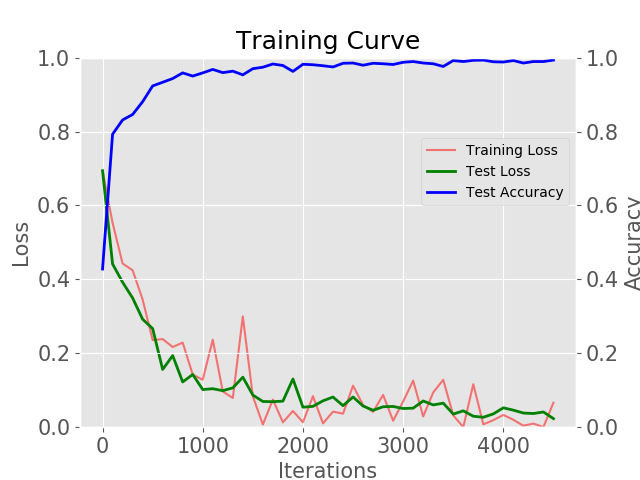
\includegraphics[width=2.4in]{entrenamiento}
	\caption{ Graph of the Training Process }
	\label{fig_sim}
	\end{figure}
	
\section{Test}

\begin{comment}	
Para esta etapa, consideramos otro dataset con 202 imagenes de plantas de maiz en la etapa V3-V7 y 202 dos imagenes de mala hierba obtenidas en campos de maiz diferentes a los que pertenecen al dataset de entrenamiento, para esta prueba se ha medido los tiempos de clasificacion promedio de diez clasificaciones de este dataset en los distintos hardwares que poseemos, empezamos con la clasificacion en Caffe sin modificaciones de software. Los resultados fueron comparados entre la red cNET de 64 y 16 filtros y se muestran en la siguiente Tabla
\end{comment}	

For this stage, another dataset with 202 images of maize plants in stage V3-V7 and 202 images of weed were considered, obtained in different maize crops that the training dataset. For this test and in order to have a reliable value its considered to classify ten times the dataset, so the average time of classification by image was obtained with the chosen hardware, we started the classification in Caffe without modifications in Software. The results were comparated between cNET with 64 and 16 filters and there are shown in the next Table \ref{table:4}.\\ 

\begin{table}[h!]
\centering
\begin{tabular}{|p{1.1cm}|p{1.5cm}|p{1.5cm}|p{2.1cm}|} 
 \hline
 \multicolumn{4}{ |c| }{\textbf{GPU}} \\
 \hline
 \textbf{cNET} & \textbf{Accuracy Weed} & \textbf{Accuracy Maize} & \textbf{Average time of classification/image} \\ 
 \hline 
 64 Filters & 95.05\% & 74.75\% & 2.34 ms \\ [0.75ex]
 \hline
 16 Filters & 94.55\% & 87.13\% & 951 $\mu$s \\ [0.75ex]
 \hline
 \multicolumn{4}{ |c| }{\textbf{CPU}} \\
 \hline
 \textbf{cNET} & \textbf{Accuracy Weed} & \textbf{Accuracy Maize} & \textbf{Average time of classification/image} \\ 
 \hline 
 64 Filters & 95.05\% & 74.75\% & 51.6 ms \\ [0.75ex]
 \hline
 16 Filters & 94.55\% & 87.13\% & 17.23 ms \\ [0.75ex]
 \hline
 \multicolumn{4}{ |c| }{\textbf{CPU Raspberry Pi 3}} \\
 \hline
 \textbf{cNET} & \textbf{Accuracy Weed} & \textbf{Accuracy Maize} & \textbf{Average time of classification/image} \\
 \hline 
 64 Filters & 95.05 \% & 74.75\% & 615 ms \\ [0.75ex]
 \hline
 16 Filters & 94.55\% & 87.13\% & 161 ms \\ [0.75ex]
 \hline
\end{tabular}
\caption{Test with the three types of Hardware}
\label{table:4}
\end{table}

\begin{comment}	
Como la tabla muestra, los mejores resultados en tiempos de clasificacion fueron alcanzados por el procesador por GPU, esta es la mejor opcion para clasificar una gran cantidad de imagenes, sin embargo este proyecto esta psenado para ser portable, por lo que consideramos al Raspberry Pi para el analisis del rendimiento de classificacion. Con la cNET de 64 filtros, los ersultos de tiempo de clasificacion fueron de 615 milisegundos, pero este tiempo no es optimo para nuestro objetivo que es la aproximacion de clasificacion en tiempo real. 
\end{comment}	

Like the table shown the best results in times of classification were achieved by the GPU processor, it is the best option to classificate a large amount of images however this project is thought to be portable, so the Raspberry Pi were considered for the analysis of classification performance. With cNET of 64 filters the results of time of classification was 615 miliseconds, so it time isn\'t the optimum for our objective that it is the approximation to classification in a real time.\\

\begin{comment}	
Los resultados presentados anteriormente no son definitivos, pues Caffe presenta algunas formas de optimizar la clasificacion de datasets de imagenes, para este documento se ha utilizado el Agrupamiento de Imagenes en una sola estructura(Batch) para clasificar el dataset de cada clase en un single forward pass y la utilizacion de Multithreading a traves del software matematico OpenBLAS. Para cada hardware se volvio a compilar Caffe con OpenBLAS en lugar de Atlas y en el programa se ingresaron todas las imagenes en un vector para ser clasificado un solo grupo de imagenes por cada clase, ademas se configuro a OpenBLAS para que use 4 Nucleos del cada hardware para obtener resultados parejos, los resultados obtenidos son los siguientes. 
\end{comment}	

The results shown previously are not definitive because Caffe has ways to optimize the classification of datasets of images, for this document batching was used to classify the dataset of each class in a single forward pass and the use of Multithreading by OpenBLAS math software. For each hardware, Caffe were recompiled with OpenBLAS instead of Atlas, in the program all images  were entered in a vector to be classified in an only batch per each class, also OpenBLAS was configured to use the 4 cores of each hardware to obtain fair results, the obtained results are the following \\ 

\begin{table}[h!]
\centering
\begin{tabular}[c c c c]{|p{2.2 cm}|p{1.1cm}|p{1.1cm}|p{2.4cm}|} 
 \hline
 \textbf{Hardware } & \textbf{Accuracy Weed} & \textbf{Accuracy Maize} & \textbf{Average time of classification/image}\\ 
 \hline 
 GPU & 89.11\% & 92.08\% & 1.58 ms \\ [0.95ex]
 \hline
 CPU & 89.11\% & 92.08\% & 10.92 ms \\ [0.95ex]
 \hline
 CPU(Raspberry Pi) & 89.11\% & 92.08\% & 150.8 ms \\ [0.95ex]
 \hline
\end{tabular}
\caption{Test of cNET 16 filters with optimized software}
\label{table:5}
\end{table}

\begin{comment}	
Los resultados muestran que para el tiempo de Clasificacion por GPU ha empeorado un 66\%, principalmente debido a que la Libreria de OpenBLAS hace extenso uso de los hilos del CPU causando que no todos los parametros seran computados por GPU como en la anterior prueba. En cambio, cuando se utiliza el CPU los resultados son mejores, debido a que las operaciones se ejecutan utilizando cada uno de los nucleos disponibles, en el caso de la CPU se noto un 22\% y para 6.3\% para el Raspberry Pi
\end{comment}	

The results show that for the GPU Classification time it has worsened by 66 \%, mainly because the OpenBLAS Library makes extensive use of the CPU threads causing that not all parameters will be computed by GPU as in the previous test. Instead, when the CPU is used the results are better, because the operations are executed using each of the four cores, in the case of the CPU we notice a 22 \% and for 6.3 \% for the Raspberry Pi \\
	
\begin{comment}	
Ahora para comparar todos estos resultados tomando en cuenta que una imagen capturada por la camara a una altura de 1,5 m puede enfocar un aproximado de 6 plantas de maiz, y segun la cantidad de mala hierba, se considerara un promedio de 12 plantas, dando un total de 18 plantas aproximadamente. Con esto se analiza cuantos frames por segundo seria lo adecuado para la adquisicion de imagenes.
\end{comment}	
Now to compare all these results taking into account that an image captured by the camera at a height of 1.5 m can focus an approximate 6 plants of maize, and according to the amount of weed, an average of 12 plants, Giving a total of about 18 plants. This analyzes how many frames per second would be appropriate for the acquisition of images.
\begin{table}[h!]
\centering
\begin{tabular}[c c c c]{|p{1.1 cm}|p{1.7cm}|p{1.7cm}|p{2.0cm}|} 
 \hline
 \textbf{Parameter} &\textbf{GPU(Without Threading) } & \textbf{CPU with Threading} & \textbf{RaspBerry Pi 3 with Threading} \\ 
 \hline 
 Time(s) & 0.0171 & 0.196 & 7.714  \\ [0.95ex]
 \hline
 FPS & 58.47  & 5.08 & 0.36  \\ [0.95ex]
 \hline
\end{tabular}
\caption{Test of a complete image and the frames per second}
\label{table:5}
\end{table}




	
	% An example of a floating figure using the graphicx package.
	% Note that \label must occur AFTER (or within) \caption.
	% For figures, \caption should occur after the \includegraphics.
	% Note that IEEEtran v1.7 and later has special internal code that
	% is designed to preserve the operation of \label within \caption
	% even when the captionsoff option is in effect. However, because
	% of issues like this, it may be the safest practice to put all your
	% \label just after \caption rather than within \caption{}.
	%
	% Reminder: the "draftcls" or "draftclsnofoot", not "draft", class
	% option should be used if it is desired that the figures are to be
	% displayed while in draft mode.
	%
	%\begin{figure}[!t]
	%\centering
	%\includegraphics[width=2.5in]{myfigure}
	% where an .eps filename suffix will be assumed under latex, 
	% and a .pdf suffix will be assumed for pdflatex; or what has been declared
	% via \DeclareGraphicsExtensions.
	%\caption{Simulation results for the network.}
	%\label{fig_sim}
	%\end{figure}
	
	% Note that the IEEE typically puts floats only at the top, even when this
	% results in a large percentage of a column being occupied by floats.
	
	
	% An example of a double column floating figure using two subfigures.
	% (The subfig.sty package must be loaded for this to work.)
	% The subfigure \label commands are set within each subfloat command,
	% and the \label for the overall figure must come after \caption.
	% \hfil is used as a separator to get equal spacing.
	% Watch out that the combined width of all the subfigures on a 
	% line do not exceed the text width or a line break will occur.
	%
	%\begin{figure*}[!t]
	%\centering
	%\subfloat[Case I]{\includegraphics[width=2.5in]{box}%
	%\label{fig_first_case}}
	%\hfil
	%\subfloat[Case II]{\includegraphics[width=2.5in]{box}%
	%\label{fig_second_case}}
	%\caption{Simulation results for the network.}
	%\label{fig_sim}
	%\end{figure*}
	%
	% Note that often IEEE papers with subfigures do not employ subfigure
	% captions (using the optional argument to \subfloat[]), but instead will
	% reference/describe all of them (a), (b), etc., within the main caption.
	% Be aware that for subfig.sty to generate the (a), (b), etc., subfigure
	% labels, the optional argument to \subfloat must be present. If a
	% subcaption is not desired, just leave its contents blank,
	% e.g., \subfloat[].
	
	
	% An example of a floating table. Note that, for IEEE style tables, the
	% \caption command should come BEFORE the table and, given that table
	% captions serve much like titles, are usually capitalized except for words
	% such as a, an, and, as, at, but, by, for, in, nor, of, on, or, the, to
	% and up, which are usually not capitalized unless they are the first or
	% last word of the caption. Table text will default to \footnotesize as
	% the IEEE normally uses this smaller font for tables.
	% The \label must come after \caption as always.
	%
	%\begin{table}[!t]
	%% increase table row spacing, adjust to taste
	%\renewcommand{\arraystretch}{1.3}
	% if using array.sty, it might be a good idea to tweak the value of
	% \extrarowheight as needed to properly center the text within the cells
	%\caption{An Example of a Table}
	%\label{table_example}
	%\centering
	%% Some packages, such as MDW tools, offer better commands for making tables
	%% than the plain LaTeX2e tabular which is used here.
	%\begin{tabular}{|c||c|}
	%\hline
	%One & Two\\
	%\hline
	%Three & Four\\
	%\hline
	%\end{tabular}
	%\end{table}
	
	
	% Note that the IEEE does not put floats in the very first column
	% - or typically anywhere on the first page for that matter. Also,
	% in-text middle ("here") positioning is typically not used, but it
	% is allowed and encouraged for Computer Society conferences (but
	% not Computer Society journals). Most IEEE journals/conferences use
	% top floats exclusively. 
	% Note that, LaTeX2e, unlike IEEE journals/conferences, places
	% footnotes above bottom floats. This can be corrected via the
	% \fnbelowfloat command of the stfloats package.




\section{Conclusion}

\begin{comment}	
-Este paper estudia una red neuronal convolucional para la clasificacion entre maiz y mala hierba, para lo cual se utilizo algunas arquitecturas de red, de donde la que proporciono mejores resultados fue la Cnet, con un 97.26\% de presicion en el entrenamiento al usar un datasetc de 44580 imagenes conteniendo las dos clases. \\
\end{comment}	

In this paper  we have studied the application of Convolutional Neuronal Networks for Classification between Maize and Weed Plants, for that we have used some CNN Architectures, the Network with best results in precision was cNET, with a 97.23 \% of accuracy of training, using a dataset of both classes of 44580 segmented images. \\

\begin{comment}	
Para buscar un procesamiento apropiado para trabajar en tiempo real, se experimento reduciendo el numero de filros de las capas de la red desde 64 hasta 16, logrando con esto disminuir el numero de parametros a ser computados durante la clasificacion, obteniendo tambien un tiempo de procesamiento de 2,5 veces menor al de la red original, este cambio tuvo un bajo impacto en la precision de entrenamiento de la red, pues este valor cayo en un 1\%, con respecto a la red original.
\begin{end}	

In order to search a right processing to work in real time, we have experimented to reduce the number of filters of the Layers of the Net from 64 to 16 filters, achiveiving to reduce the number of parameters to be computed during the classification , we obteined a classification time 2.5 times less than the original Net of 64 filters , this change had a small impact in the training accuracy of the net, it value increased 1 \% in comparation with the original net. \\

\begin{comment}	
-Ademas nuestros experimentos al utilizar diferentes procesadores, demostraron que se obtienen mejores resultados en cuanto a velocidad al trabajar con una a tarjeta grafica ENVIDIA que posee soporte CUDA debido a su arquitectura de computacion paralela, siendo este 10 veces mas rapido que el CPU normal y 100 veces mas rapido que una RaspBerry Pi3.
\end{comment}	

Also, by using different methods to classify the images in our experiments, the results showed that the best time of classification was achieved by using a Nvidia Graphic Cards, this is due the Parallel Architecture that this GPU has and also it has fully support for the computation platform CUDA, it demostrated to be 18 times faster than a normal CPU and 170 times faster than a Raspberry Pi 3. \\

\begin{comment}	
-El estudio demostro que es mejor obtener las imagenes para el dataset realizar algunos giros en las imagenes de las plantas del dataset, debido a que esto aporta mejoras en la identificacion de plantas, pues estas siempre tienen orientaciones diferentes.
\end{comment}	

The study demostrated that is better to perform some geometrical tranformations to the Dataset images due it benefits to improve the classification of plants because the plants ever have different orientations in the crop field. \\

-El uso de Multithreading y Batching a traves de la libreria OpenBLAS es muy beneficioso en el caso de usar CPU, aumentando la rapidez de procesamiento en el porcentaje superior al 20\%, con la Rasberry pi, se obtuvo una minima mejora, en cambio fue pejudicial con el uso de GPU , pues provoca que la rapidez se reduzca considerablemente. \\

-The use of Multithreading and Batching through the library OpenBLAS is very beneficial in the case of using CPU, increasing the speed of processing in the percentage higher than 20 \%, with the Rasberry pi, a minimum improvement was obtained, instead it was pejudicioal with the use of GPU, because it causes that the speed is reduced considerably. \\



   





% conference papers do not normally have an appendix


% use section* for acknowledgment
\section*{Acknowledgment}
\begin{comment}	
-Damos gracias a la Graja Agroecologica y Demostrativa de Pillaro y a dueños de cultivos de maiz de lugares aledaños. que nos permitieron tomar muestras de plantas ,para la obtencion del dataset del proyecto.

-Este trabajo ha sido apoyada por la Universidad de las Fuerzas Armadas ESPE Extension Latacunga. 
\end{comment}	

The authors would like to thank to the "Granja Agroecol\'ogica y Demostrativa" of P\'illaro City and owners of corn crops of the city which allowed us to take samples of plants, to conform the dataset of this project. \\

This work has been supported by the University of the Army "ESPE" Latacunga. 


% trigger a \newpage just before the given reference
% number - used to balance the columns on the last page
% adjust value as needed - may need to be readjusted if
% the document is modified later
%\IEEEtriggeratref{8}
% The "triggered" command can be changed if desired:
%\IEEEtriggercmd{\enlargethispage{-5in}}

% references section

% can use a bibliography generated by BibTeX as a .bbl file
% BibTeX documentation can be easily obtained at:
% http://mirror.ctan.org/biblio/bibtex/contrib/doc/
% The IEEEtran BibTeX style support page is at:
% http://www.michaelshell.org/tex/ieeetran/bibtex/
%\bibliographystyle{IEEEtran}
% argument is your BibTeX string definitions and bibliography database(s)
%\bibliography{IEEEabrv,../bib/paper}
%
% <OR> manually copy in the resultant .bbl file
% set second argument of \begin to the number of references
% (used to reserve space for the reference number labels box)

\bibliographystyle{IEEEtran}
\bibliography{bibliografiapaper}




% that's all folks
\end{document}


